%%%%%%%%%%%%%%%%%%%%%%%%%%%%%%%%%%%%%%%%%
% Short Sectioned Assignment
% LaTeX Template
% Version 1.0 (5/5/12)
%
% This template has been downloaded from:
% http://www.LaTeXTemplates.com
%
% Original author:
% Frits Wenneker (http://www.howtotex.com)
%
% License:
% CC BY-NC-SA 3.0 (http://creativecommons.org/licenses/by-nc-sa/3.0/)
%
%%%%%%%%%%%%%%%%%%%%%%%%%%%%%%%%%%%%%%%%%

%----------------------------------------------------------------------------------------
%	PACKAGES AND OTHER DOCUMENT CONFIGURATIONS
%----------------------------------------------------------------------------------------

\documentclass[paper=a4, fontsize=11pt]{scrartcl} % A4 paper and 11pt font size

\usepackage{graphicx}

%\usepackage[T1]{fontenc} % Use 8-bit encoding that has 256 glyphs
%\usepackage{fourier} % Use the Adobe Utopia font for the document - comment this line to return to the LaTeX default
\usepackage[english]{babel} % English language/hyphenation%
\usepackage{amsmath,amsfonts,amsthm} % Math packages

\usepackage{lipsum} % Used for inserting dummy 'Lorem ipsum' text into the template

\usepackage{sectsty} % Allows customizing section commands
\allsectionsfont{\normalfont\scshape} % Make all sections centered, the default font and small caps

\usepackage{fancyhdr} % Custom headers and footers
\pagestyle{fancyplain} % Makes all pages in the document conform to the custom headers and footers
\fancyhead{} % No page header - if you want one, create it in the same way as the footers below
\fancyfoot[L]{} % Empty left footer
\fancyfoot[C]{} % Empty center footer
\fancyfoot[R]{\thepage} % Page numbering for right footer
\renewcommand{\headrulewidth}{0pt} % Remove header underlines
\renewcommand{\footrulewidth}{0pt} % Remove footer underlines
\setlength{\headheight}{13.6pt} % Customize the height of the header

\numberwithin{equation}{section} % Number equations within sections (i.e. 1.1, 1.2, 2.1, 2.2 instead of 1, 2, 3, 4)
\numberwithin{figure}{section} % Number figures within sections (i.e. 1.1, 1.2, 2.1, 2.2 instead of 1, 2, 3, 4)
\numberwithin{table}{section} % Number tables within sections (i.e. 1.1, 1.2, 2.1, 2.2 instead of 1, 2, 3, 4)

\setlength\parindent{0pt} % Removes all indentation from paragraphs - comment this line for an assignment with lots of text

%----------------------------------------------------------------------------------------
%	TITLE SECTION
%----------------------------------------------------------------------------------------

\newcommand{\horrule}[1]{\rule{\linewidth}{#1}} % Create horizontal rule command with 1 argument of height

\title{	
\normalfont \normalsize 
\textsc{[CS/DS 864] Machine Learning - 1 project} \\ [25pt] % Your university, school and/or department name(s)
\horrule{0.5pt} \\[0.4cm] % Thin top horizontal rule
\huge Photo Triage Benchmark \\ % The assignment title
\horrule{2pt} \\[0.5cm] % Thick bottom horizontal rule
}

\author{Darshan Bhat - MT2015038\\Keerthan Pai K - MT2015053} % Your name

\date{\normalsize\today} % Today's date or a custom date



\begin{document}

\maketitle % Print the title

\section{Problem}

People often take a series of nearly redundant pictures to capture a moment or scene. However, selecting photos to keep or share from a large collection is a painful chore. To address this problem, we seek a relative quality measure within a series of photos taken of the same scene, which can be used for automatic photo triage. Towards this end,  a large dataset comprised of photo series distilled from personal photo albums have been gathered. By augmenting the dataset with ground truth human preferences among photos within each series, the problem is to establish a benchmark for measuring the effectiveness of algorithmic approaches to modeling human preferences.

\newpage
\section{Exploratory analysis of the dataset}

The dataset contains 15,545 unedited photos distilled from personal photo albums. The photos are organized in 5,953 series. For each series, human preferences are collected by a crowd-sourced user study. The following figure shows several example series, annotated with human preferences.
\\
\begin{figure}[h]
  \centering
  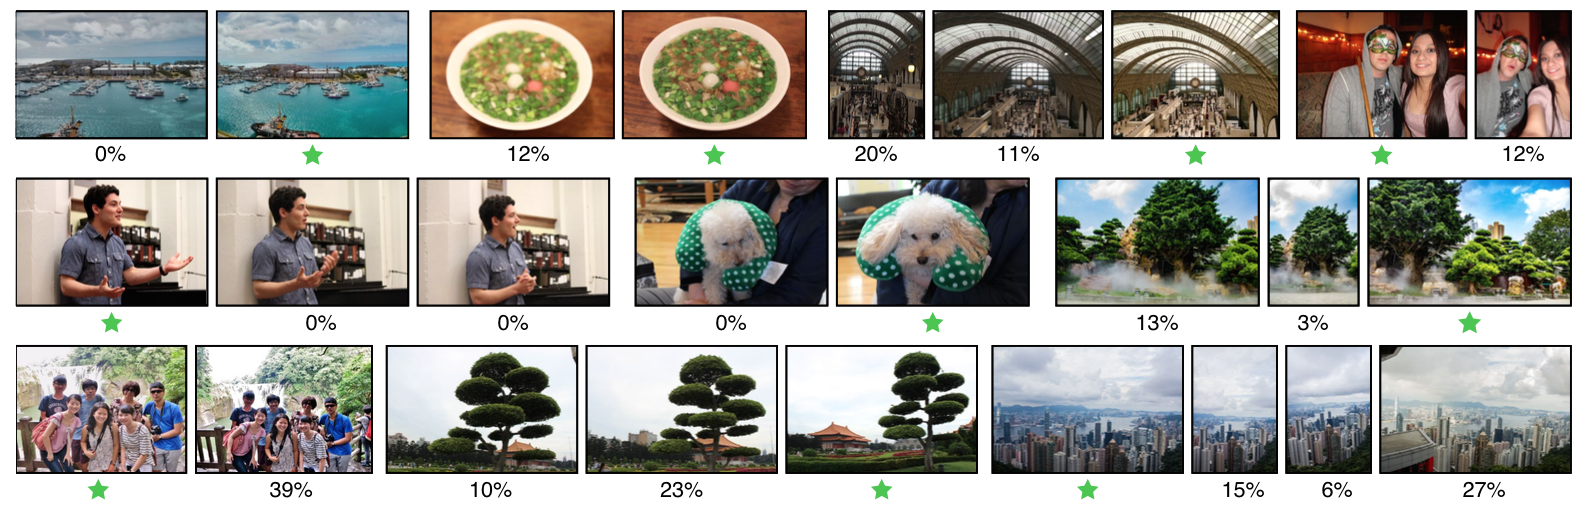
\includegraphics[width=6in]{AdobeProblem.png}
  \caption[Photo Triage]
   {Photo Triage: The photo with the green star in each series is the one preferred by the majority of people, while the percentage below each other photo indicates what fraction of people would prefer that photo over the starred one in the same series. }
\end{figure}
\\
Out of the 5,953 series, 4560 are randomly sampled for training, 195 for validation, and the remaining 967 for testing. 
The dataset includes the following folders and files:

\begin{itemize}
        \item $\bold{train\_pairlist.txt}$ lists the pairs in all training photo series.\\The format is "$\#SERIES\_ID$  $\#PHOTO1\_IND$  $\#PHOTO2\_IND$ \\$\#PREFERENCE\_RATIO\_of\_PHOTO1\_OVER\_PHOTO2$\\ $\#RANK\_of\_PHOTO1 RANK\_of\_PHOTO2$"

        \item $\bold{val\_pairlist.txt}$ list all the pairs in all validation photo series. To test the performance of learning the human preferences offline, save the result of the predictor into a textfile and run test.m. The result could be either binary or float for the preferene of PHOTO1 over PHOTO2 for each pair.

 \item $\bold{train\_val\_series.mat}$ lists more information about the testing photo series, such as the Bradley-Terry scores modelled from human preferences.
 
 \item $\bold{train\_val\_imgs/}$ includes all the images which are resized in 800x800 with its aspect ratio preserved. The format is "$\#SERIES\_ID(\%06d)-\#PHOTO\_IND(\%02d).JPG$".
\end{itemize}

\newpage

\section{Algorithmic Approach}
Many hand tuned features like color, lighting, composition, clarity, SIFT features can be considered for the problem. But as suggested in the website, feature extracted from pre-trained network like AlexNet, VGGNet will tend to outperform the hand tuned features. We will use pre-trained ConvNet to extract the features.

\paragraph{}
The training images belong to different categories like nature, selfie, indoor, outdoor etc. So the training using single image features will not make sense and will not lead to convergence. Rather we will take two images from the series of similar images and use the difference of their individual features as a new feature for training. Features are extracted from two exactly same ConvNets for two different images in a pair(each feature of around 4096 values). A new feature is formed by taking the difference of these two feature vector. This new feature is then used to train a new model with binary output denoting which image is the better of the two.

\paragraph{}
So we will process the images pairwise to predict the better image among the two. This result can be then clubbed to decide the overall best image of the series.


\subsection*{Model Description:}

\paragraph{}
The input of our model is a pair of images ($I_1$, $I_2$). We aim at learning a function p:IxI $\mapsto$ {-1,1} where 1 means the first image is better and -1 means the opposite. The model p should be skew symmetric, that is, if the input images are flipped, the output should also flip, p($I_1$,$I_2$) = -p($I_2$,$I_1$)


\end{document}